\chapter{Relèvement}

Dans le cas du cylindre, on a $\alpha_1=0$, ce qui conduit à ce que $\rot \mathbf{b}=0$ et donc $\mathbf{a}=\grad\psi^0$.

\section{Gradient dans $\HH^1$}
\label{impGradh1}
\subsection{Implémentation}
Si l'on veut utiliser le problème (\ref{pbpsi0}) dans $\HH^1$, alors il faut utiliser un multiplicateur de Lagrange pour ajouter une contrainte sur $\psi^0$, par exemple $\int \psi^0 = 0$. Cela se traduit par le changement de formulation variationnelle suivant où l'on cherche $(\psi^0,\lambda)\in \HH^1\times\R$ et où $(\varphi,\nu)$ est la fonction de test :
\[ \int_\Omega\grad \psi^0\grad\varphi + \int_\Omega \psi^0\nu + \int_\Omega \lambda\varphi = \int_{\partial\Omega} \alpha_0\varphi \]
On va donc créé un espace de fonction produit correspondant à $\HH^1\times\R$.

\lstinputlisting[linerange={space}]{../../src/psi0.hpp}

On ajoute une fonction permettant de rajouter en option le profil d'entrée en fonction du rayon et de la vitesse. Cela correspond à $\alpha_0$.

\lstinputlisting[linerange={option}]{../../src/psi0.cpp}

Une fois les éléments de l'espace créé, on peut définir la forme bilinéaire de la façon suivante :

\lstinputlisting[linerange={bilinear}]{../../src/psi0.cpp}

Ici, $u$ correspond à $\psi^0$ et $v$ à $\varphi$ et \texttt{inner} est le produit scalaire.\\

On veut que ce qui rentre du cylindre par l'entrée, correspondant à la partie du maillage marquée 1, sorte par l'autre bout du cylindre, marqué 2, et que le tour du cylindre, marqué 3, soit imperméable. Ce qui donne la terme de droite suivant :

\lstinputlisting[linerange={rhs}]{../../src/psi0.cpp}

Une fois le problème résolut, on veut projeter le gradient de $\psi^0$ sur $\LL^2$. Pour cela on résout le problème simple $u=\grad\psi^0$ qui mène à la forme variationnelle suivante :
\[ \int_\Omega \bm{u}\cdot\bm{v} = \int_\Omega \grad\psi^0\cdot\bm{v} \]

\lstinputlisting[linerange={gradpsi0}]{../../src/psi0.cpp}

\subsection{Résultats}
Dans les figure \ref{az},\ref{aIn},\ref{aOut}, on peut observer $\bm{a}$ dans le cylindre. Ici, $\alpha_1=0$ et 
\[ \alpha_0(x,y)= \begin{cases} -2\times v\times\left(1-\frac{x^2+y^2}{r^2}\right) &\mbox{sur } \Gamma_1\\
2\times v\times\left(1-\frac{x^2+y^2}{r^2}\right)&\mbox{sur } \Gamma_2\\
0 &\mbox{sur } \Gamma_3 \end{cases} \]

\begin{figure}[H]
\centering
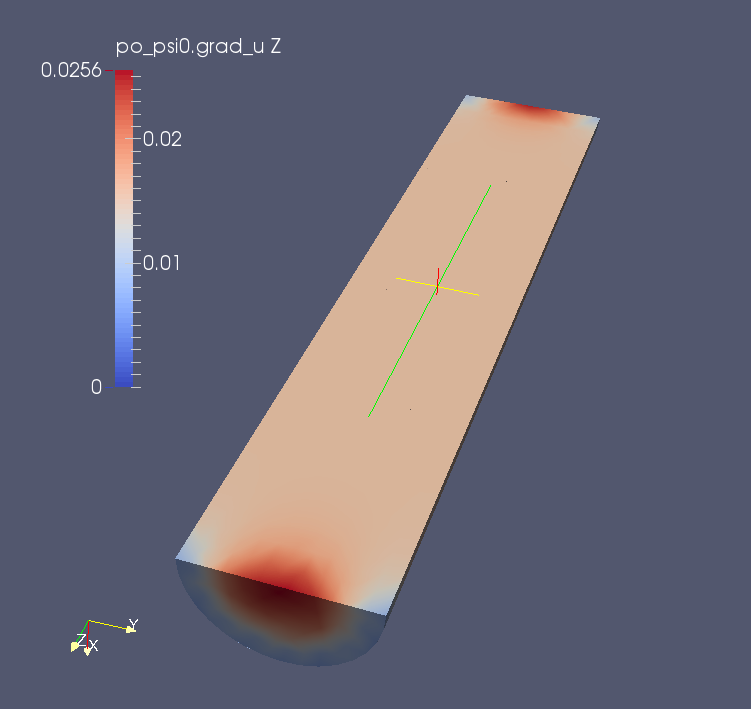
\includegraphics[scale=0.35]{az}
\caption{composante $z$ de $\bm{a}$}
\label{az}
\end{figure}
\begin{figure}[H]
\centering
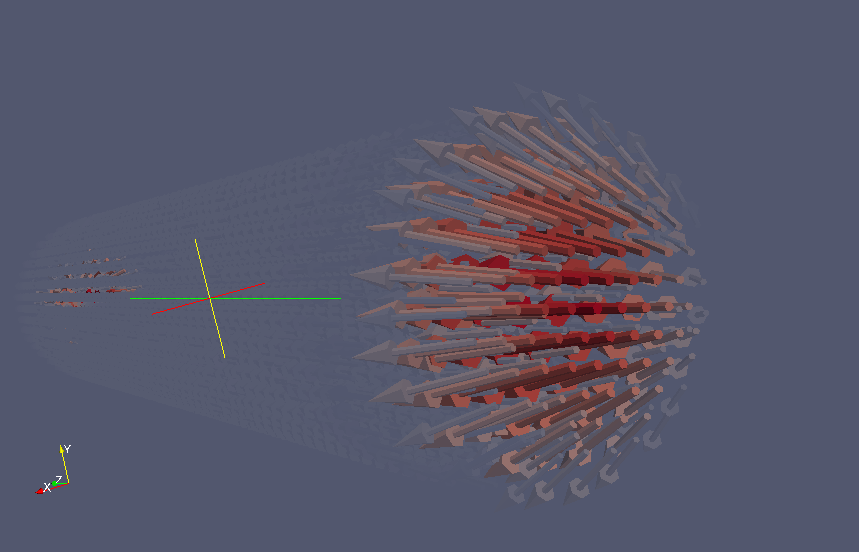
\includegraphics[scale=0.5]{aIn}
\caption{entrée du cylindre}
\label{aIn}
\end{figure}
\begin{figure}[H]
\centering
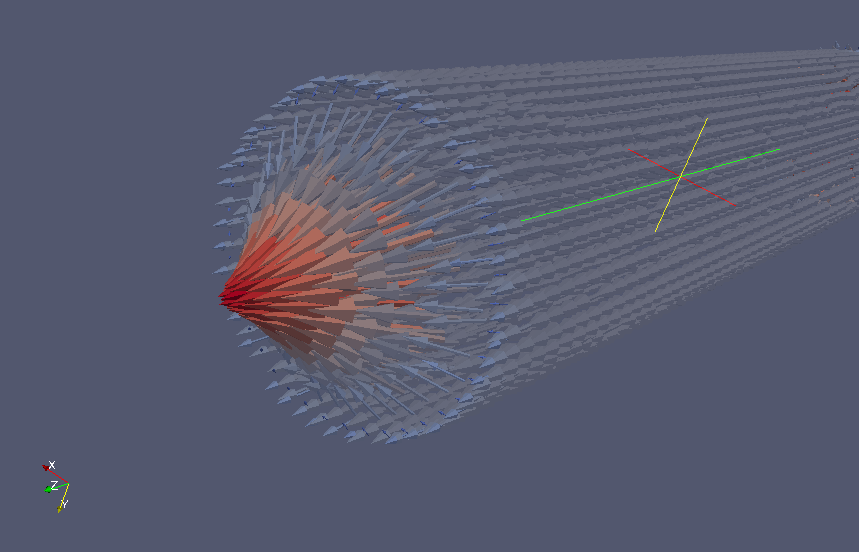
\includegraphics[scale=0.5]{aOut}
\caption{sortie du cylindre}
\label{aOut}
\end{figure}

%\section{Gradient dans $\HH(div)$}

%%% Local Variables:
%%% TeX-master: "../report.tex"
%%% eval: (flyspell-mode 1)
%%% ispell-local-dictionary: "french"
%%% End:
